\subsection{Data collector}
	La componente \textit{data collector} permette di trasferire i dati prodotti dai singoli gateway ed inviati nei vari topic di Kafka, all'interno di un database di tipo \glock{timeseries}.
	\newline
	Allo stesso tempo, permette di filtrare i dati collezionati ed inviare dei messaggi di avviso, all'interno di un apposito topic, nel caso in cui vengano rilevati dei valori anomali.
	\newline
	Il filtraggio dei dati viene fatto a partire dagli alert impostati all'interno della \glock{web app} e salvati in un database relazionale (\glock{PostgreSQL}).
	\begin{itemize}
		\item La componente è stata sviluppata in Java 11.
	\end{itemize}
	
		\subsubsection{Diagramma dei package}%%%%%%%%%OK
		\begin{figure}[H]
				\centering
				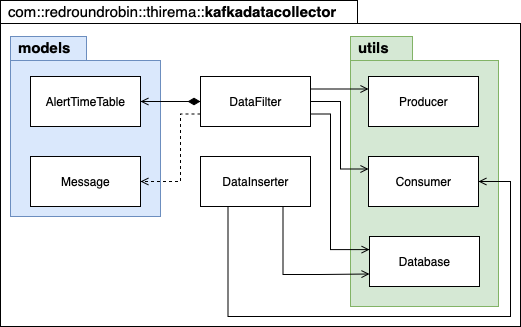
\includegraphics[scale=0.600]{res/images/DATACOLLECTOR/Packagekafkadatacollector.png}
				\caption{Diagramma dei package della componente data collector}
				\label{Diagramma 5}
			\end{figure}
		\subsubsection{Dipendenze esterne}
			La componente ha due dipendenze esterne:
			\begin{itemize}
				\item \textbf{KafkaProducer<K, V>}, classe concreta che implementa l'interfaccia Producer<K,V>. Svolge il compito di client per il cluster \glock{kafka}, pubblicando dati all'interno di un topic. La classe DataFilter ne possiede un riferimento.
				\item \textbf{KafkaConsumer<K,V>}, classe concreta che implementa l'interfaccia Consumer<K,V>. Svolge il compito di client per il cluster Kafka, consumando i messaggi resenti all'interno di uno o più topic. La classi DataInserter e DataFilter ne possiedono un riferimento.	
			\end{itemize}	
		\begin{landscape}
		\subsubsection{Diagramma delle classi}%%%%%%%%%%%%%%%%%%%%%%%OK
			\begin{figure}[H]
				\centering
				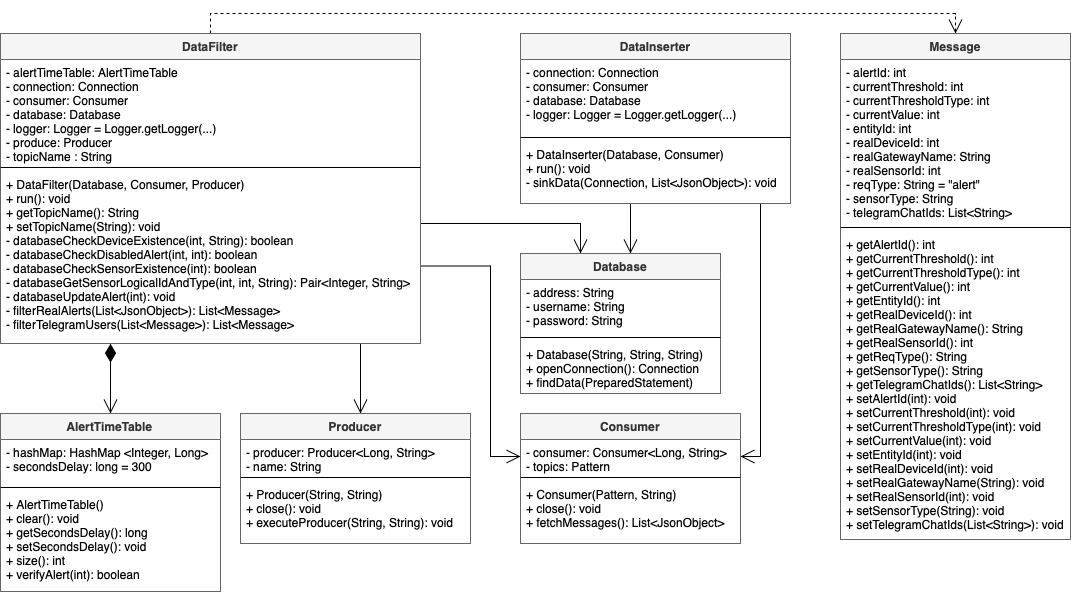
\includegraphics[scale=0.550]{res/images/DATACOLLECTOR/ClassikafkaDataCollector.png}
				\caption{Diagramma delle classi della componente data collector}
				\label{Diagramma 6}
			\end{figure}
		Come si vede nel diagramma sono presenti le seguenti classi:
		\begin{itemize}
			\item \textbf{Database}: rappresenta un database; i suoi campi propri sono infatti lo username, la password e l'indirizzo del database che rappresenta;
			\item \textbf{Consumer}: rappresenta un consumer di Kafka, che è infatti contenuto al suo interno. La classe viene utilizzata per "consumare" messaggi da uno o più topic di Kafka (in questo caso dai topic contenenti i dati reperiti tramite i vari gateway presenti nel sistema); 
			\item \textbf{Producer}: rappresenta un producer di Kafka, che è infatti contenuto al suo interno. La classe viene utilizzata per "produrre" messaggi contenenti messaggi di alert all'interno di un apposito topic;
			\item \textbf{DataInserter}: è una classe al cui interno è presente un riferimento alla classe Database (che rappresenta \glock{Timescale} in questo caso) ed alla classe Consumer. Il suo compito è quello di reperire i dati da tutti i topic collegati ad un gateway ed inserirli all'interno del database non relazionale;
			\item \textbf{DataFilter}: classe che contiene oltre che un riferimento a Database (che rappresenta Postgre) e a Consumer, anche un riferimento a Producer e AlertTimeTable; questo perché DataFilter dopo aver filtrato i dati, grazie ai suoi metodi (e grazie alla classe AlertTimeTable), inserisce i messaggi derivati dai dati consumati direttamente in un topic Kafka tramite un producer;
			\item \textbf{AlertTimeTable}: classe utilizzata per definire e far rispettare un certo delay tra l'invio di un messaggio di alert ed un messaggio successivo. Questo limite è stato fissato solo per avvisi di uno stesso sensore.
			\item \textbf{Message}: rappresenta un messaggio di alert inviato da DataFilter all'interno di un topic adibito questa funzione. Contiene infatti tutte le informazioni necessarie alle API per inviare un messaggio ad uno o più utenti iscritti, tramite la Web-app, alla ricezione di quel determinato alert.
		\end{itemize}
		\end{landscape}
		\begin{landscape}
		\subsubsection{Diagrammi di sequenza}%%%%%%%%%OK
			\begin{figure}[H]
				\centering
				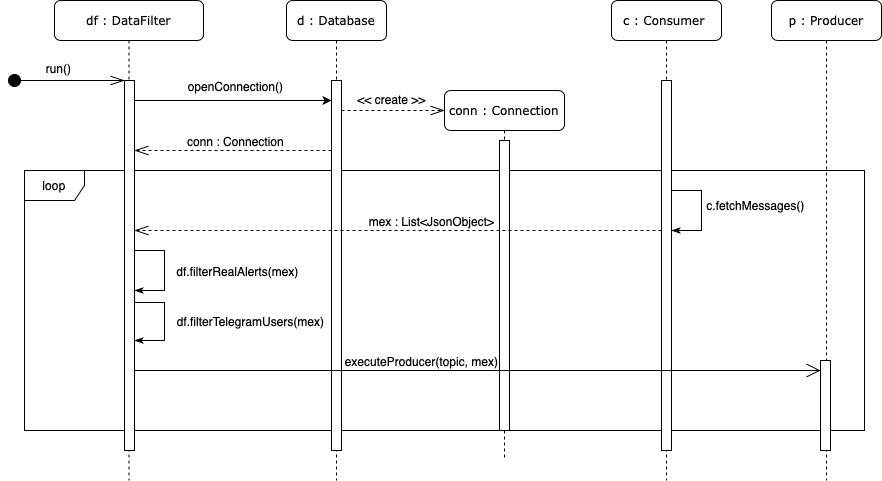
\includegraphics[scale=0.550]{res/images/DATACOLLECTOR/DataFilter.ThreadsKafkaDataCollector.png}
				\caption{Diagramma di sequenza in cui viene mostrato il funzionamento del filtraggio dati nella componente data collector}
				\label{Diagramma 7}
			\end{figure}
			Come si evince dal diagramma in alto, funzionamento di DataFilter è il seguente:
			\begin{itemize}
				\item DataFilter apre la connessione con il database relazionale Postgre;
				\item vengono quindi estratti i dati dai topic \glock{Kafka} collegati ai gateway;
				\item i valori vengono filtrati, garantendo che dispositivo e sensore siano presenti nel database e che i valori rilevati superino effettivamente la soglia;
				\item i valori vengono filtrati nuovamente per verificare che gli utenti a cui dovrebbero arrivare abbiano configurato il \glock{bot Telegram} correttamente;
				\item infine vengono prodotti un insieme di messaggi di alert che, tramite un produttore vengono inseriti nel topic \glock{kafka} "alerts". 
			\end{itemize}
			\begin{figure}[H]
				\centering
				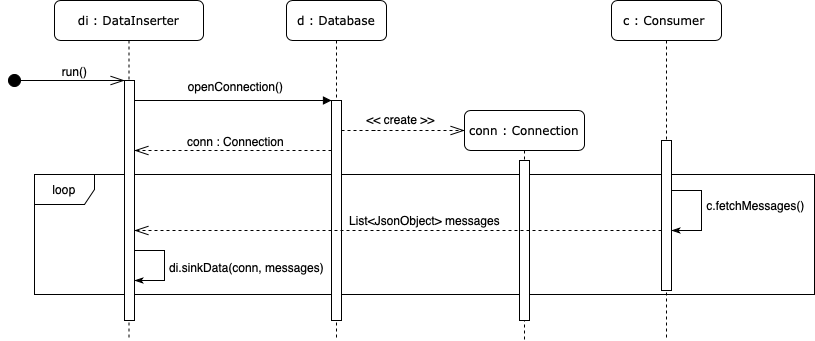
\includegraphics[scale=0.550]{res/images/DATACOLLECTOR/DataInserter.ThreadsKafkaDataCollector.png}
				\caption{Diagramma di sequenza in cui viene mostrato il funzionamento dell'inserimento dati nella componente data collector}
				\label{Diagramma 8}
			\end{figure}
			Il comportamento di DataInserter è il seguente:
			\begin{itemize}
				\item DataInserter apre una connessione con il database \glock{Timescale};
				\item ogni qualvolta il suo Consumer trova dei nuovi dati nei topic collegati ai gateway, vengono inviati i messaggi al DataInserter;
				\item DataInserter infine inserisce i dati all'interno del database.
			\end{itemize}
	\end{landscape}